\documentclass[12pt,titlepage]{article}
\usepackage[margin=1.25in]{geometry}
\usepackage{graphicx,amsmath,blindtext,minted}

%% Variables definition
\newcommand{\vSubject}{Data Structure and Algorithm Practicum}
\newcommand{\vSubtitle}{Class and Object}
\newcommand{\vName}{Muhammad Baihaqi Aulia Asy'ari}
\newcommand{\vNIM}{2241720145}
\newcommand{\vClass}{1I}
\newcommand{\vDepartment}{Information Technology}
\newcommand{\vStudyProgram}{D4 Informatics Engineering}

%% [START] Tikz related stuff
\usepackage{tikz}
\usetikzlibrary{svg.path,calc,shapes.geometric,shapes.misc}
\tikzstyle{terminator} = [rectangle, draw, text centered, rounded corners = 1em, minimum height=2em]
\tikzstyle{preparation} = [chamfered rectangle, chamfered rectangle sep=0.75em, draw, text centered, minimum height = 2em]
\tikzstyle{process} = [rectangle, draw, text centered, minimum height=2em]
\tikzstyle{decision} = [diamond, aspect=2, draw, text centered, minimum height=2em]
\tikzstyle{data}=[trapezium, draw, text centered, trapezium left angle=60, trapezium right angle=120, minimum height=2em]
\tikzstyle{connector} = [line width=0.25mm,->]
%% [END] Tikz related stuff

%% [START] Fancy header related stuff
\usepackage{fancyhdr}
\pagestyle{fancy}
\setlength{\headheight}{15pt} % compensate fancyhdr style
\fancyhead{}
\fancyfoot{}
\fancyfoot[L]{\thepage}
\fancyfoot[R]{\textit{\vSubject - \vSubtitle}}
\renewcommand{\footrulewidth}{0.4pt}% default is 0pt, overline for footer
%% [END] Fancy header related stuff

%% [START] Custom tabular command related stuff
\usepackage{tabularx}
\newcommand{\details}[2]{
    #1 & #2  \\
}
%% [END] Custom tabular command related stuff

%% [START] Figure related stuff
\newcommand{\image}[3][1]{
    \begin{figure}[h]
        \centering
        \includegraphics[#1]{#2}
        \caption{#3}
        \label{#3}
    \end{figure}
}
%% [END] Figure related stuff

%%
\usepackage{pgf-umlcd}

\renewcommand{\umldrawcolor}{black}
\renewcommand{\umlfillcolor}{white}
%%

\begin{document}
\begin{titlepage}
    \centering
    \vfill
    {\bfseries\LARGE
        \vSubject\\
        \vskip0.25cm
        \vSubtitle
    }
    \vfill
    
\includegraphics[width=6cm]{images/polinema-logo.png}
    \vfill
    {
        \textbf{Name}\\
        \vName\\
        \vskip0.5cm
        \textbf{NIM}\\
        \vNIM\\
        \vskip0.5cm
        \textbf{Class}\\
        \vClass\\
        \vskip0.5cm
        \textbf{Department}\\
        \vDepartment\\
        \vskip0.5cm
        \textbf{Study Program}\\
        \vStudyProgram
    }
\end{titlepage}

\newpage

\section*{11.Question}

\begin{enumerate}
    \item {
        Class/Object has a caracteristic of having attributes and methods.
    }
    \item {
        To declare a class, the key word to be use is \texttt{class}.
    }
    \item {
        There are 4 total attributes, 2 of them are string and the other are integer. the attributes name are namaBarang, jenisBarang, stok, and hargaSatuan.
    }
    \item {
        The attributes were declared on line 4 and line 5.
    }
    \item {
        There are 4 methods inside the class 3 of them are void methods and one of them is string method.
    }
    \item {
        The methods were declared on line 7 until line 22.
    }
    \item {
        \begin{minted}[autogobble]{java}
            void kurangiStok(int n) {
                if (stok <= 0) {
                    stok = stok - n;
                }
            }
        \end{minted}
    }
    \item {
        The integer parameter is a variable to be used in the mathematical operation in the function and must be in a form of integer to perform the mathematical operation.
    }
    \item {
        Because the function of \texttt{hitungHargaTotal()} has an output from the calculation of total price in a form of integer.
    }
    \item {
        Because \texttt{tambahStok()} only change the value of a variable and does not need to output a value.
    }
    \item {
        The instantiation process happend at line 5 and the object created is named \texttt{b1}
    }
    \item {
        To access the attributes and methods of the object \texttt{b1}, write \texttt{b1.methods()} or \texttt{b1.attributes}
    }
    \item {
        The parametric constructor in the class Barang in part 4 was declared in line 9 until line 14
    }
    \item {
        In line 16 of class BarangMain in part 4, what the code is doing is instantiate an object called b2 using the parametric constructor
    }
    \item {
        \begin{minted}[autogobble]{java}
            Barang b3 = new Barang("KTT Kang White", "Keyboard Switch", 9999, 3_000);
        \end{minted}
    }
\end{enumerate}

\newpage

\section*{12.Task}

\begin{enumerate}
    \item {
        \begin{minted}[autogobble]{java}
            public class Lingkaran {
                double phi = Math.PI, r;
                Lingkaran() {

                }
                Lingkaran(double r) {
                    this.r = r;
                }
                double hitungLuas() {
                    return phi * r * r;
                }
                double hitungKeliling() {
                    return 2 * r * phi;
                }
            }
        \end{minted}
    }
    \item {
        \begin{minted}[autogobble]{java}
            public class RentalTransaction {
                String memberId, memberName, gameName;
                int dailyPrice, dayRent;
                RentalTransaction() {

                }
                RentalTransaction(String memberId, String memberName, String gameName, int dailyPrice, int dayRent) {
                    this.memberId = memberId;
                    this.memberName = memberName;
                    this.gameName = gameName;
                    this.dailyPrice = dailyPrice;
                    this.dayRent = dayRent;
                }
                void print() {
                    System.out.printf("""
                            Member ID   : %s
                            Member name : %s
                            Game name   : %s
                            Price       : %d
                            Rent period : %d %s
                            Total       : %d
                            """, memberId, memberName, gameName, dailyPrice, dayRent, dayRent < 2 ? "day" : "days", dailyPrice * dayRent);
                }
            }
        \end{minted}
        -

        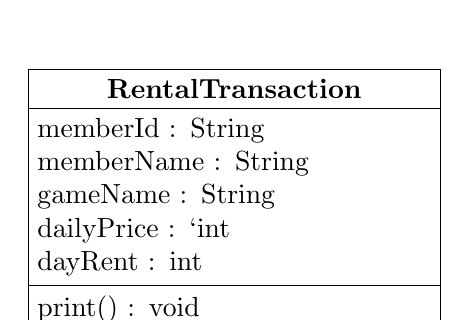
\begin{tikzpicture}
            \begin{class}[text width=5cm]{RentalTransaction}{0,0}
                \attribute{memberId : String}
                \attribute{memberName : String}
                \attribute{gameName : String}
                \attribute{dailyPrice : `int}
                \attribute{dayRent : int}
                \operation{print() : void}
            \end{class}
        \end{tikzpicture}
    }
    \item {
        \begin{minted}[autogobble]{java}
            public class Item {
                String name;
                int unitPrice, qty;

                Item() {

                }

                Item(String name, int unitPrice, int qty) {
                    this.name = name;
                    this.unitPrice = unitPrice;
                    this.qty = qty;
                }

                
                int calculateTotalPrice() {
                    return qty * unitPrice;
                }

                int calculateDiscount() {
                    int totalPrice = calculateTotalPrice();
                    if (totalPrice > 100_000) return (int) 0.9;
                    if (totalPrice > 50_000) return (int) 0.95;
                    return 1;
                }

                int calculateFinalPrice() {
                    int totalPrice = calculateTotalPrice();
                    int discount = calculateDiscount();
                    return totalPrice * discount;
                }
            }
        \end{minted}
    }

\newpage
    \item {
        \begin{minted}[autogobble]{java}
            public class PacMan {
                int x, y, height, width;
                
                PacMan() {

                }

                PacMan(int x, int y, int height, int width) {
                    this.x = x;
                    this.y = y;
                    this.width = width;
                    this.height = height;
                }

                void moveLeft() {
                    if (x > 0) x--;
                }

                void moveRight() {
                    if (x < width) x++;
                }

                void moveDown() {
                    if (y > 0) y--;
                }

                void moveUp() {
                    if (y < height) y++;
                }

                void printCoordinate() {
                    System.out.printf("x: %d y: %d", x, y);
                }
            }
        \end{minted}
    }

\end{enumerate}

\end{document}